\documentclass{article}
\usepackage[utf8]{inputenc}
\usepackage[T1]{fontenc}
\usepackage[utf8]{inputenc}
\usepackage[norsk]{babel}
\usepackage{amsmath}
\usepackage{verbatim}
\usepackage{hyperref}
\usepackage{enumerate}
\usepackage{graphicx}
\usepackage{listings}
\usepackage{color}
\usepackage{gensymb}
\usepackage{subfig}
\usepackage{fancyvrb}
\definecolor{codegreen}{rgb}{0,0.6,0}
\definecolor{codegray}{rgb}{0.5,0.5,0.5}
\definecolor{codepurple}{rgb}{0.58,0,0.82}
\definecolor{backcolour}{rgb}{0.95,0.95,0.92}
\setlength{\parindent}{0pt}
\lstdefinestyle{mystyle}{
    backgroundcolor=\color{backcolour},
    commentstyle=\color{codegreen},
    keywordstyle=\color{magenta},
    numberstyle=\tiny\color{codegray},
    stringstyle=\color{codepurple},
    basicstyle=\footnotesize,
    breakatwhitespace=false,
    breaklines=true,
    captionpos=b,
    keepspaces=true,
    numbers=left,
    numbersep=5pt,
    showspaces=false,
    showstringspaces=false,
    showtabs=false,
tabsize=2}
\lstset{style=mystyle}

\title{Oblig2 INF4300}
\author{mathiaki}


\begin{document}

\maketitle

\newpage
\tableofcontents
\newpage

\section{Texture description}
	The first thing to do in this mandatory assignment was to find the best GLCM for all 4 of the textures. In the last assignment our job was to find these matrices, but this time we already have the finished glcm matrices.\\
	
	With the finished GLCM matices, we can now get the feature images for the different orientations.\\
	\begin{figure}[h]%
		\centering
    	\subfloat[Texture]{{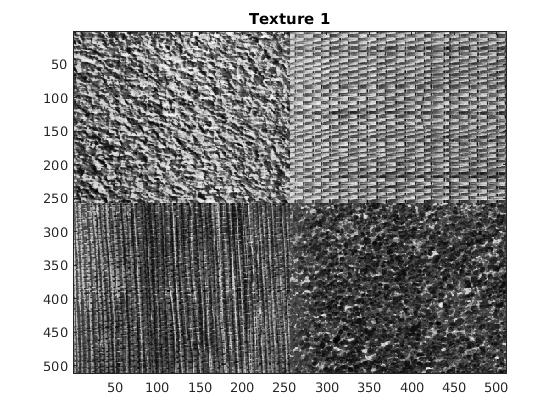
\includegraphics[width=11.5cm]{texture.jpg} }}%
    	\caption{Original texture}%
    	\label{fig:original_texture}%
	\end{figure}	
\newpage
\subsection{Matrix data}
	Included in the assignment we got some matrices with the GLCM for each texture.
	
	
	\begin{figure}[h!]%
		\centering
    	\subfloat[Texture 1]{{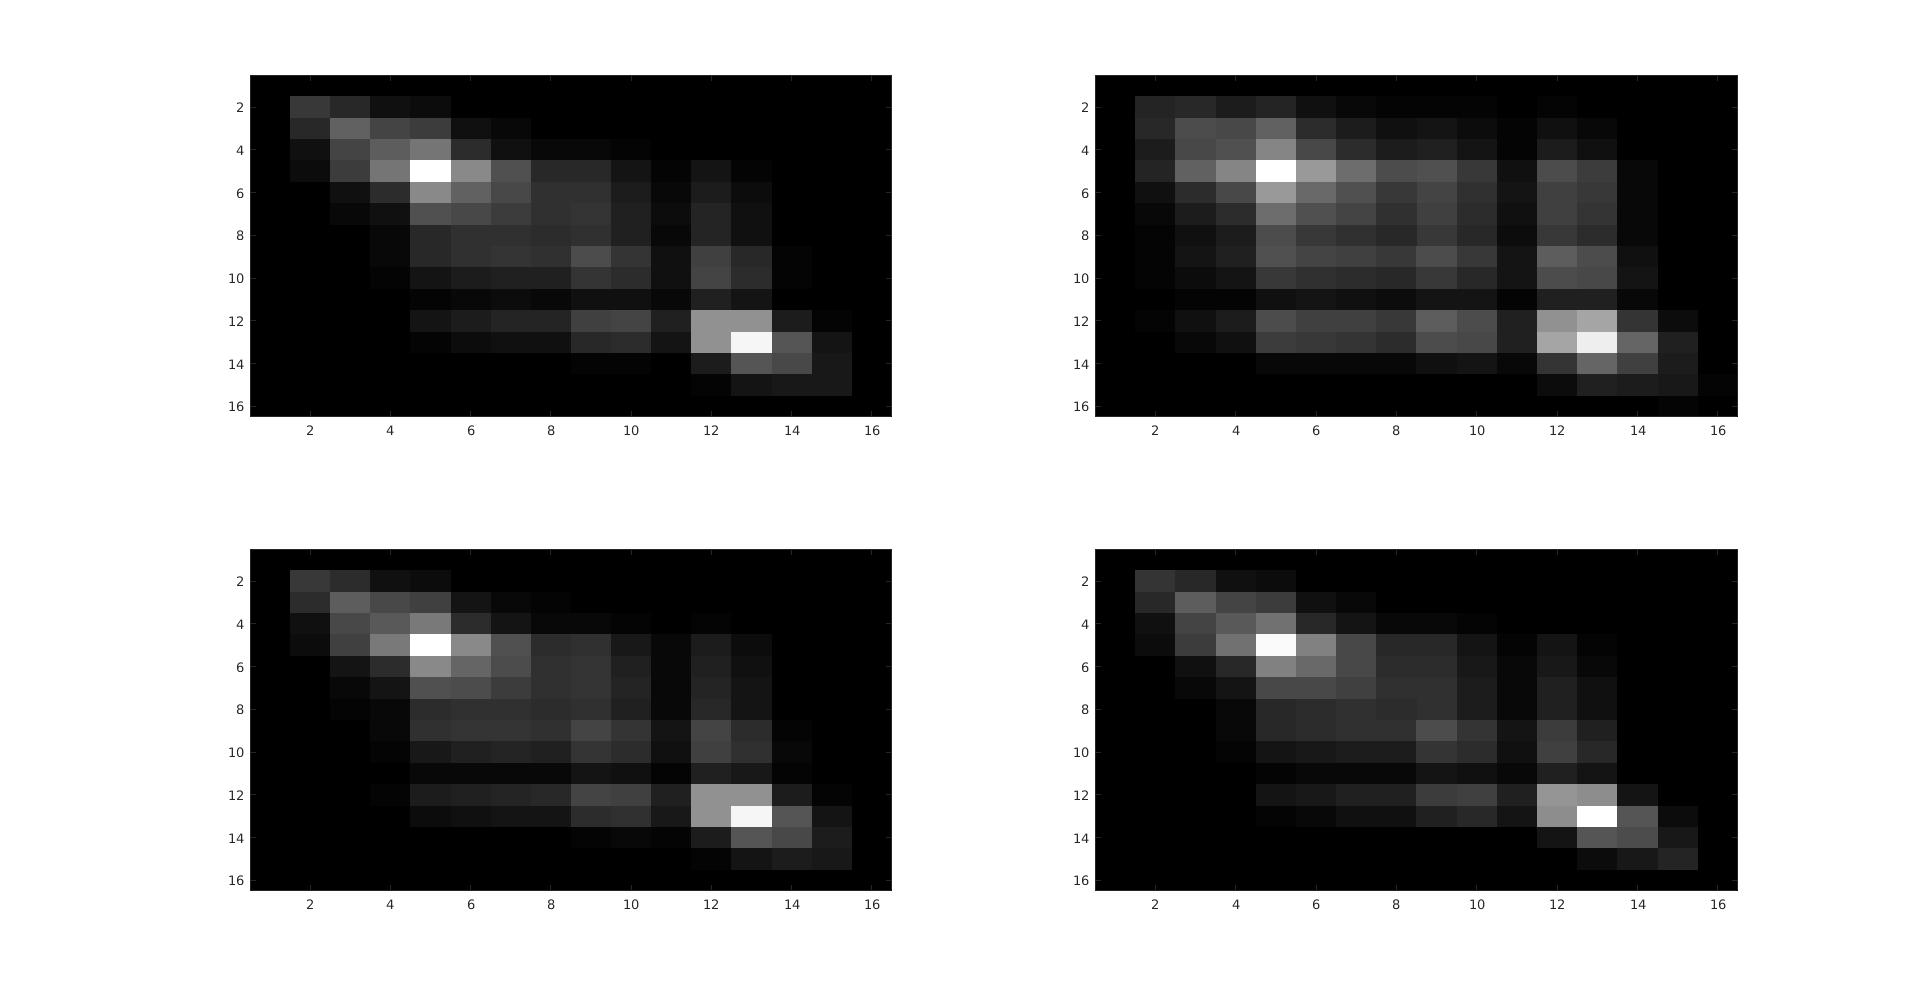
\includegraphics[width=11.5cm]{o1_f1.jpg} }}%
    	\caption{Texture 1 GLCM}%
    	\label{fig:o1_f1}%
	\end{figure}

	From this first texture we choose the second of the 4 images.\\
	This corresponds to dx=1 dy=0  


	\begin{figure}[h!]%
		\centering
    	\subfloat[Texture 2]{{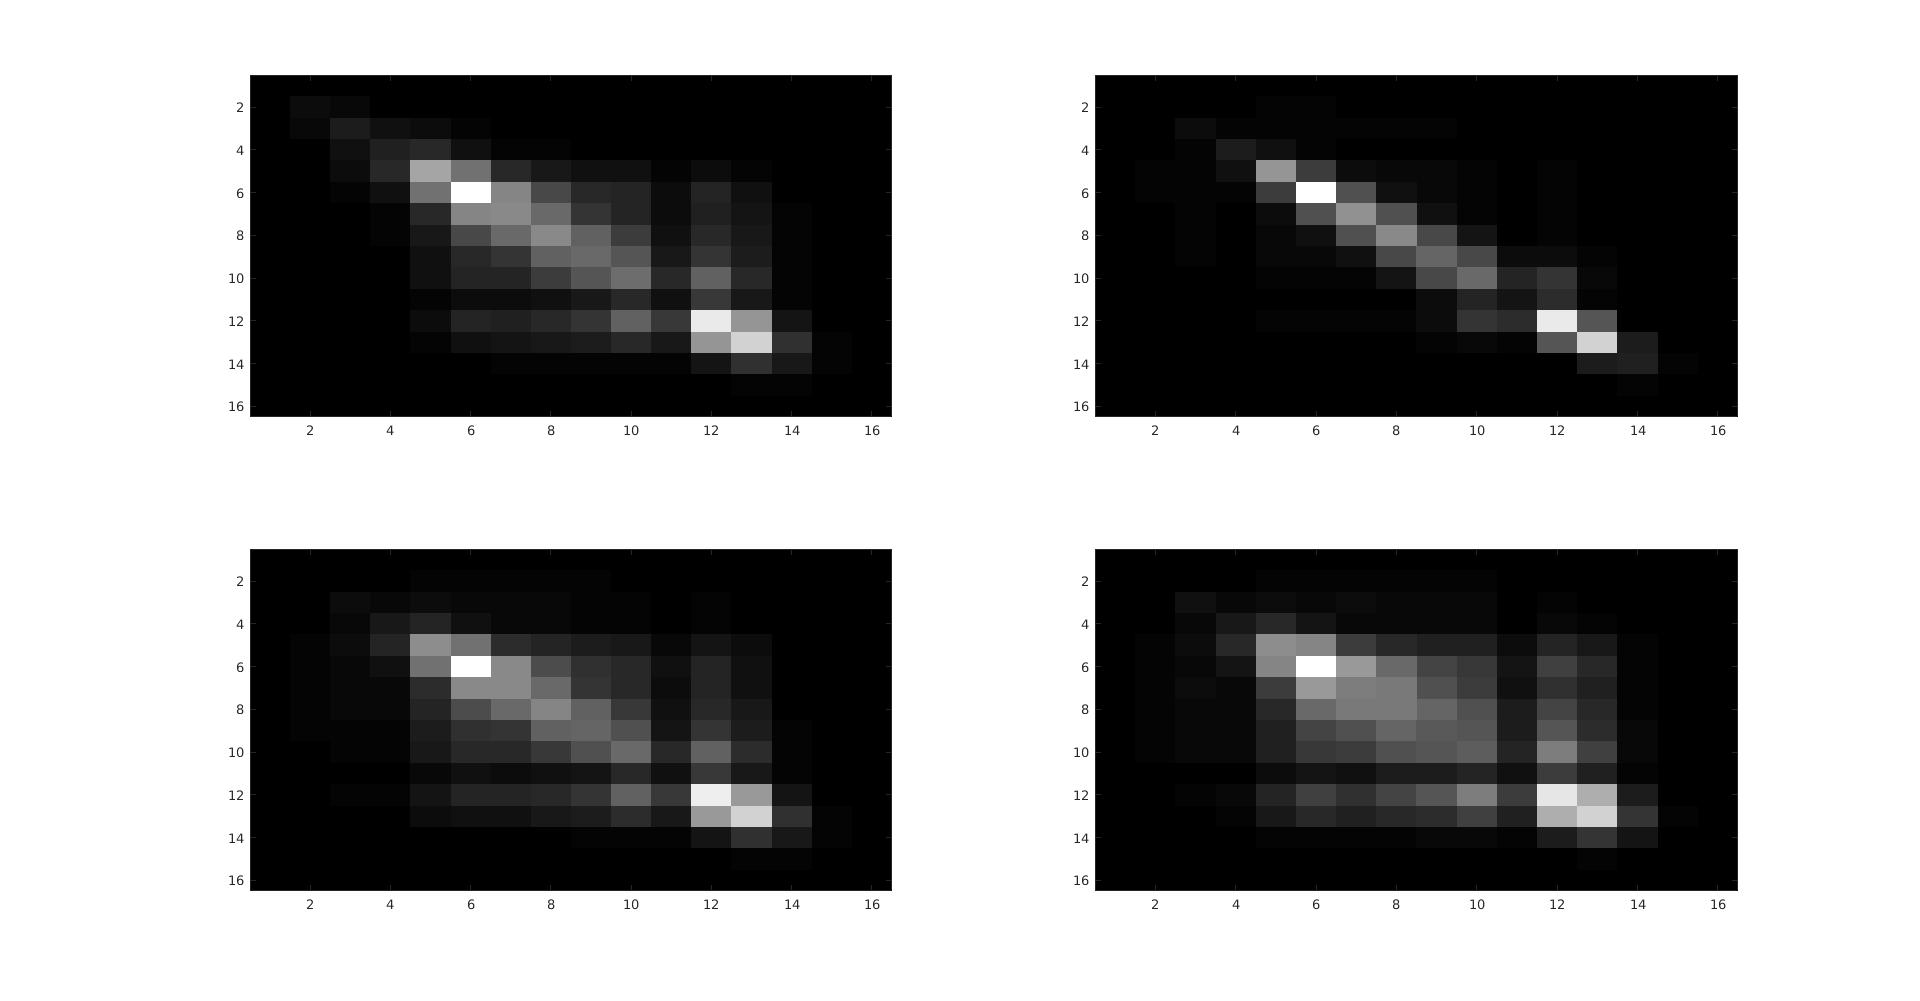
\includegraphics[width=10.5cm]{o1_f2.jpg} }}%
    	\caption{Texture 2 GLCM}%
    	\label{fig:o1_f2}%
	\end{figure}

	From this first texture we choose the first of the 4 images.\\
	This corresponds to dx=0 dy=-1  
\newpage
	\begin{figure}[h!]%
		\centering
    	\subfloat[Texture 3]{{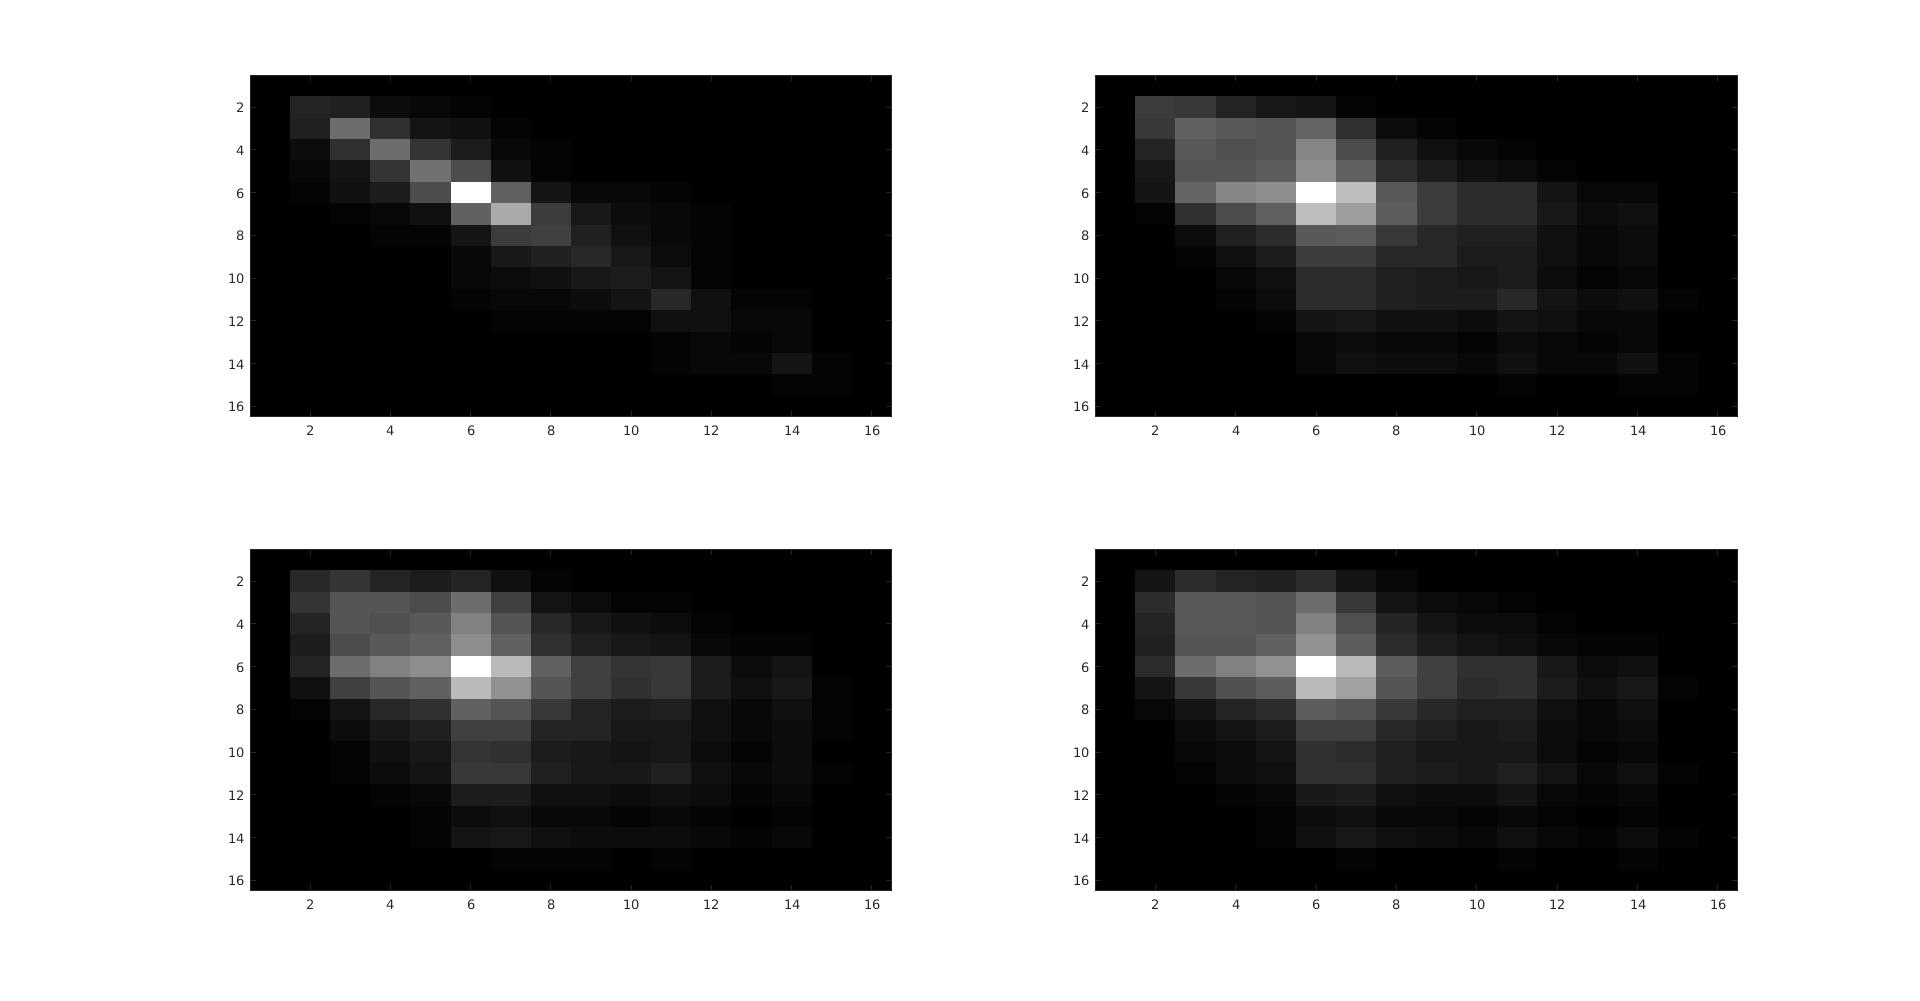
\includegraphics[width=10.5cm]{o1_f3.jpg} }}%
    	\caption{Texture 3 GLCM}%
    	\label{fig:o1_f3}%
	\end{figure}

	From this first texture we choose the first or second of the 4 images.\\
	This corresponds \textit{best} to dx=0 dy=-1  

	\begin{figure}[h!]%
		\centering
    	\subfloat[Texture 4]{{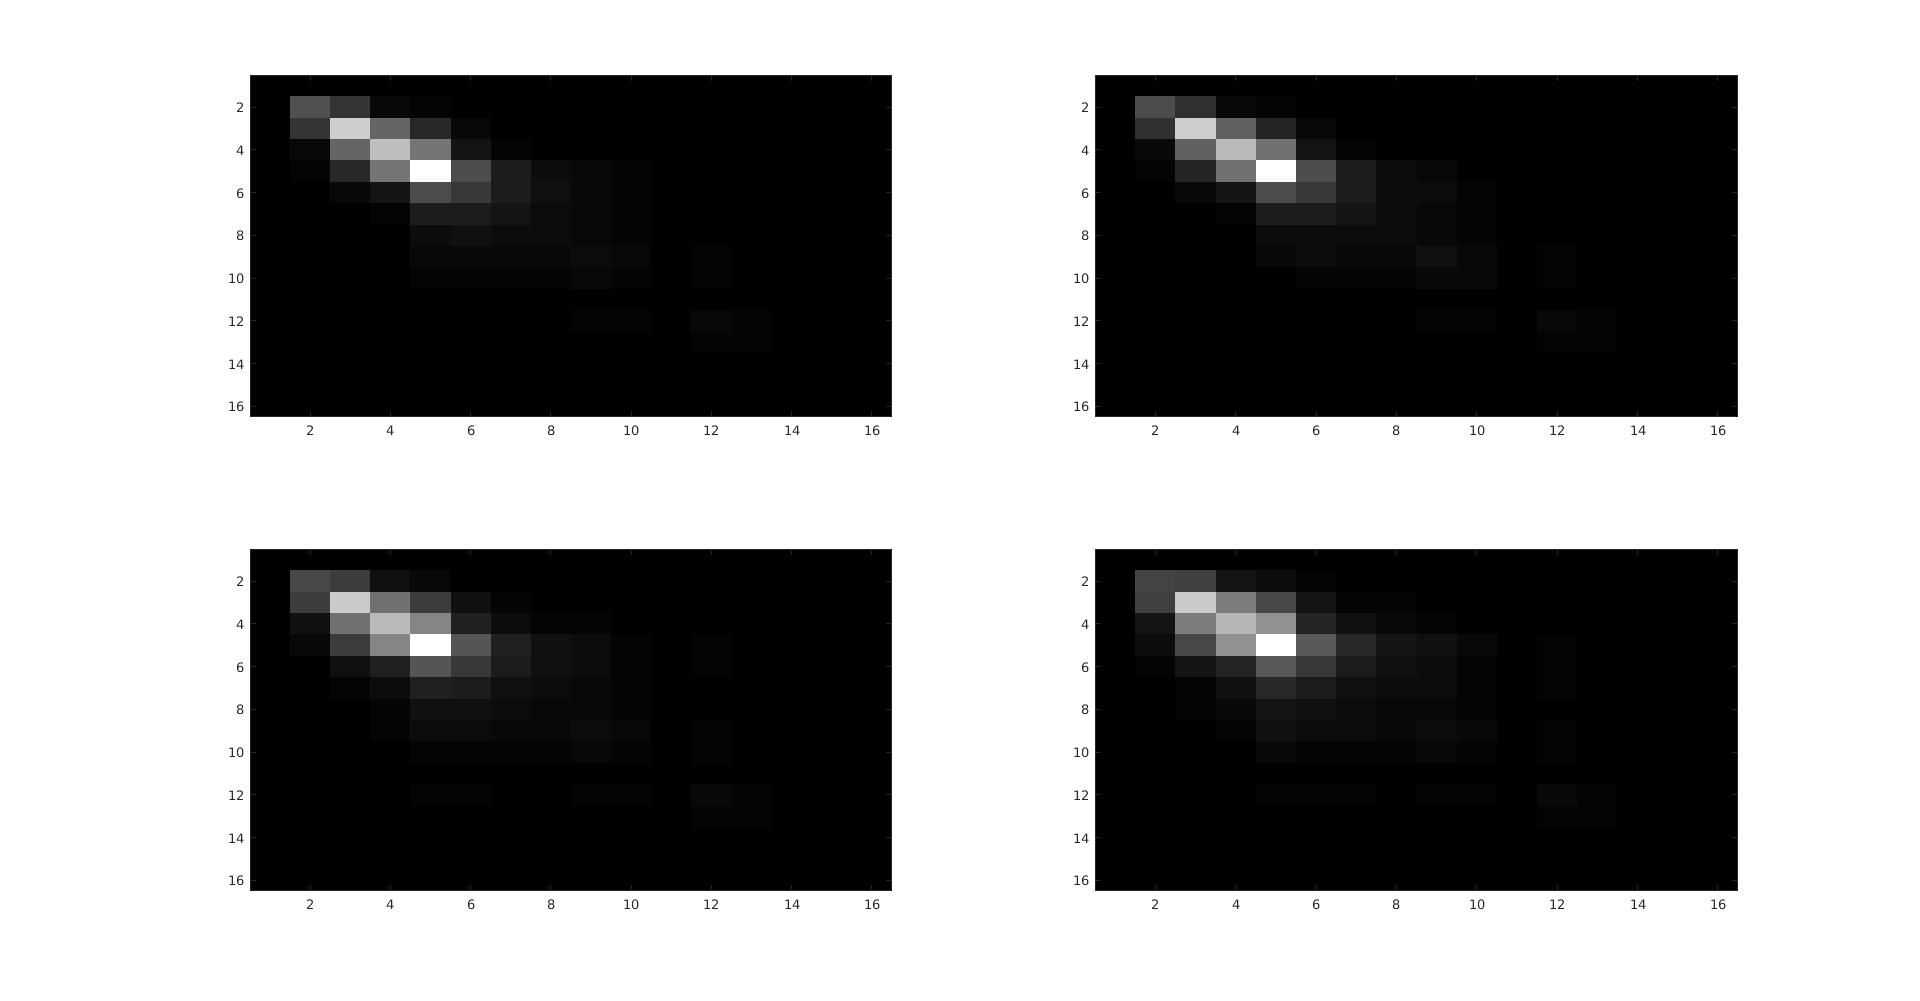
\includegraphics[width=10.5cm]{o1_f4.jpg} }}%
    	\caption{Texture 4 GLCM}%
    	\label{fig:o1_f4}%
	\end{figure}

	From this first texture we choose the first of the 4 images.\\
	This corresponds to dx=0 dy=-1

\vspace{10px}		
	
	Now that we have all the necessary dxy values, we can now start with the sliding GLCM part of the program. 

\newpage
From this point onwards we stop using the GLCM matrices from the assignment, and start making and using our own:
\lstinputlisting[language=Matlab]{../files/GLCM.m}
An important note here is that the GLCM is going to be symmetric, so Q2 and Q3 will be (close to) identical every time. The same is true for Q12 and Q13.


\newpage
\section{Quadrant and sliding}
	With the GLCM matrices from assignment 1 we can now divide the each of the GLCM matrices in to 4 parts: 

	\begin{figure}[h]
	\centering
	\begin{BVerbatim}
GLCM Gliding window
|---------------|
|Q11|Q12|       |
|---|---|  Q2   |
|Q13|Q14|       |
|-------|-------|
|       |       |
|  Q3   |  Q4   |
|       |       |
|---------------|
	\end{BVerbatim}
	\caption{GLCM Gliding matrix}%
	\label{verb:gGLCM}
	\end{figure}


When we now run the gliding GLCM the result of the different quadrants are stored in the respective variables. As shown in \ref{verb:gGLCM}.\\

As the Q1 quadrant has the most difference between the different textures, it is natural to spit the quadrant up in to 4 subquadrants.
The glidingGLCM can be found in appendix A \ref{fig:gGLCM}.



\newpage
The Q matrices was then analyzed. And at this point we had to choose how many features we want to use in the classification. We ended up with 3 features, and subsequently 3 quadrants were used:\\
\textit{Instead of showing all 8 sliding window GLCM matrices, I have chosen to only show the 3 that i used throughout the rest of the assignment.}\\


	\begin{figure}[h!]%
		\centering
    	\subfloat[Quadrant Q1]{{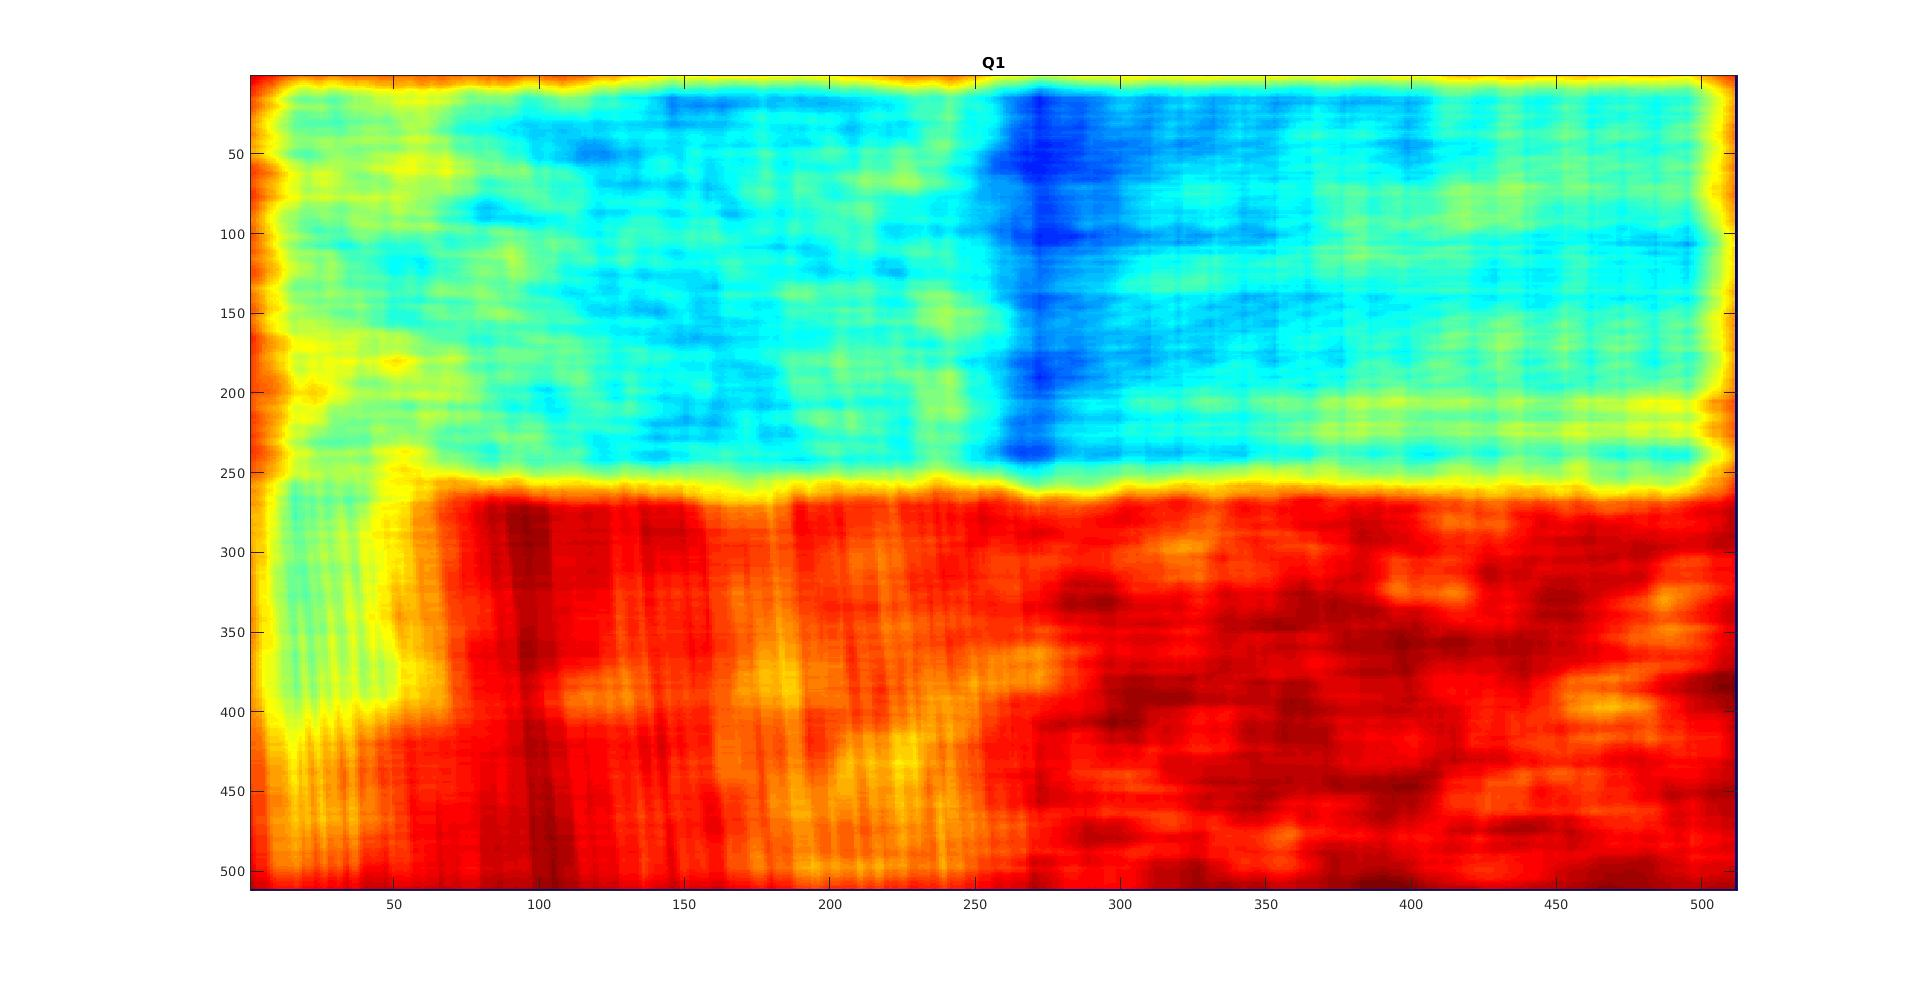
\includegraphics[width=12.5cm]{o3_q1.jpg} }}%
    	\caption{Qadrant Q1 with dx=1 and dy=0}%
    	\label{fig:o3_q1}%
	\end{figure}
The first quadrant is the top left in the GLCM. As expected is the 2 textures with the most \' black \' to \' black \' pixels hot.   
\newpage
	\begin{figure}[h!]%
		\centering
    	\subfloat[Quadrant Q4]{{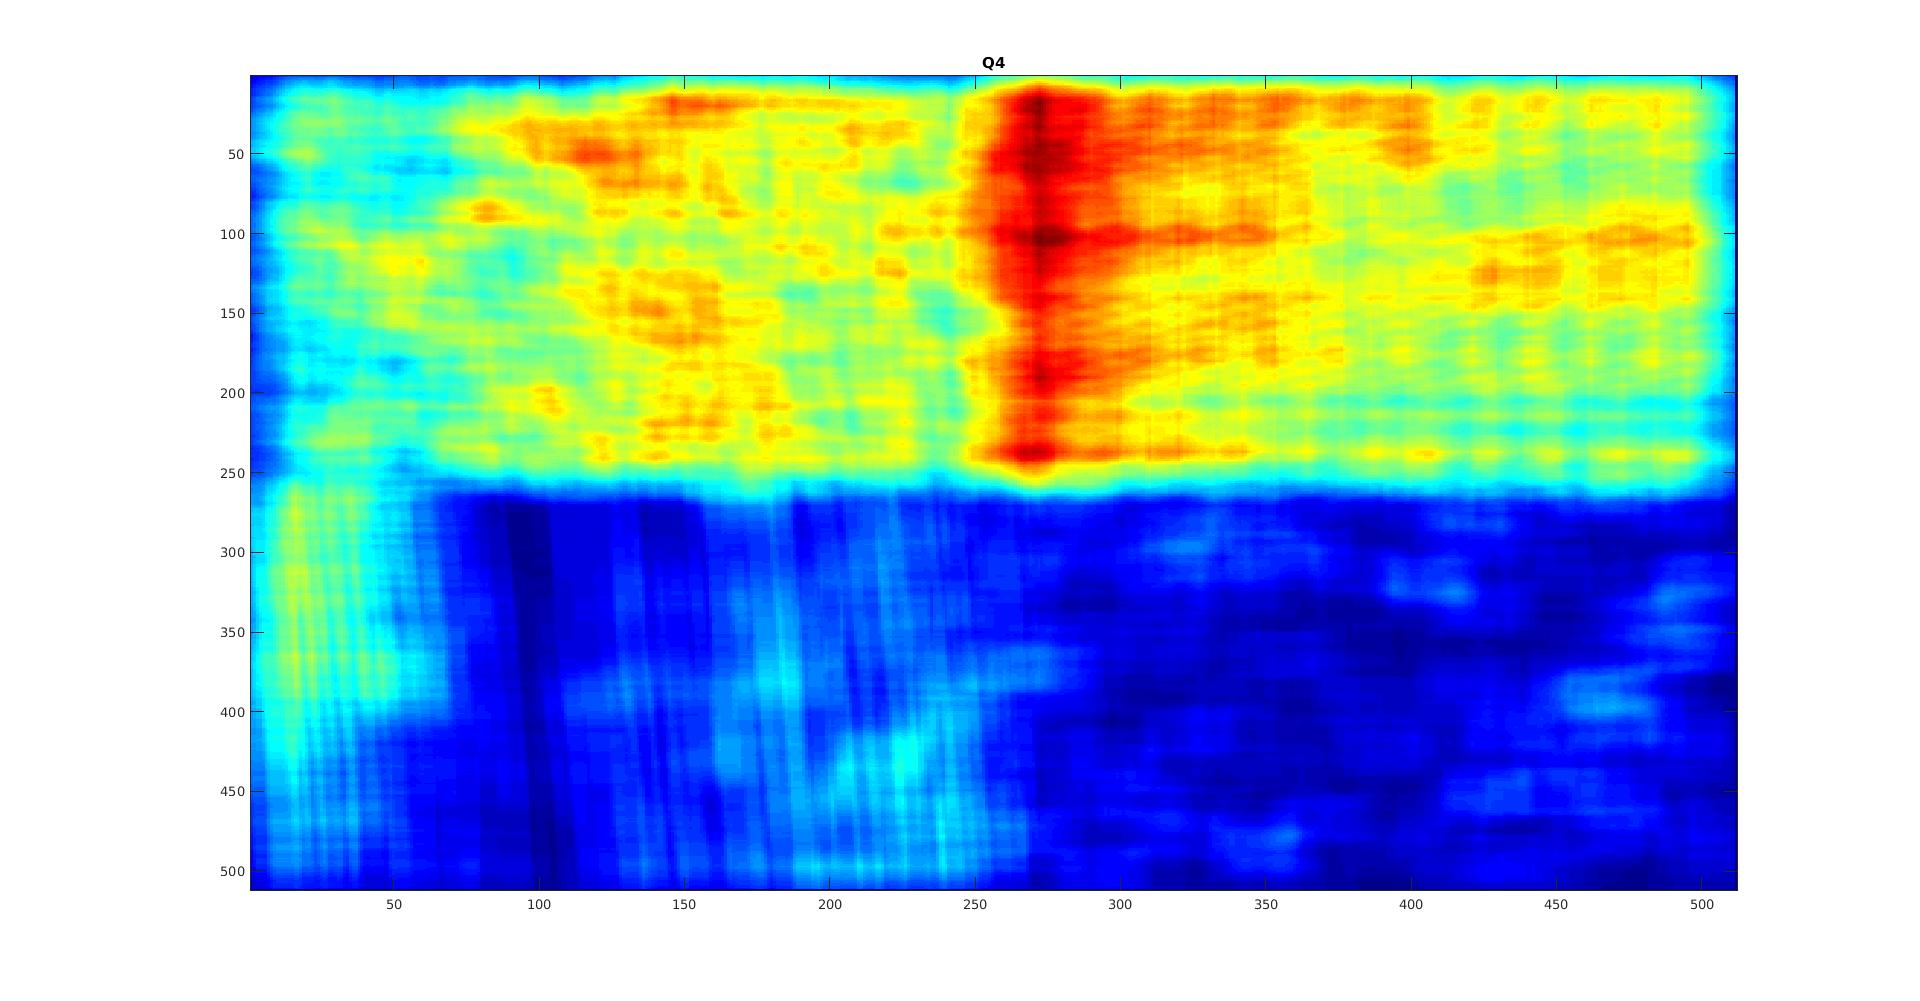
\includegraphics[width=12.5cm]{o3_q4.jpg} }}%
    	\caption{Qadrant Q4 with dx=0 and dy=-1}%
    	\label{fig:o3_q4}%
	\end{figure}
The second quadrant is almost the opposite, of the first. Here the GLCM jumps from high to high values, as it does in Q4. We have here a horizontal pattern. 
\newpage
	\begin{figure}[h!]%
		\centering
    	\subfloat[Quadrant Q12]{{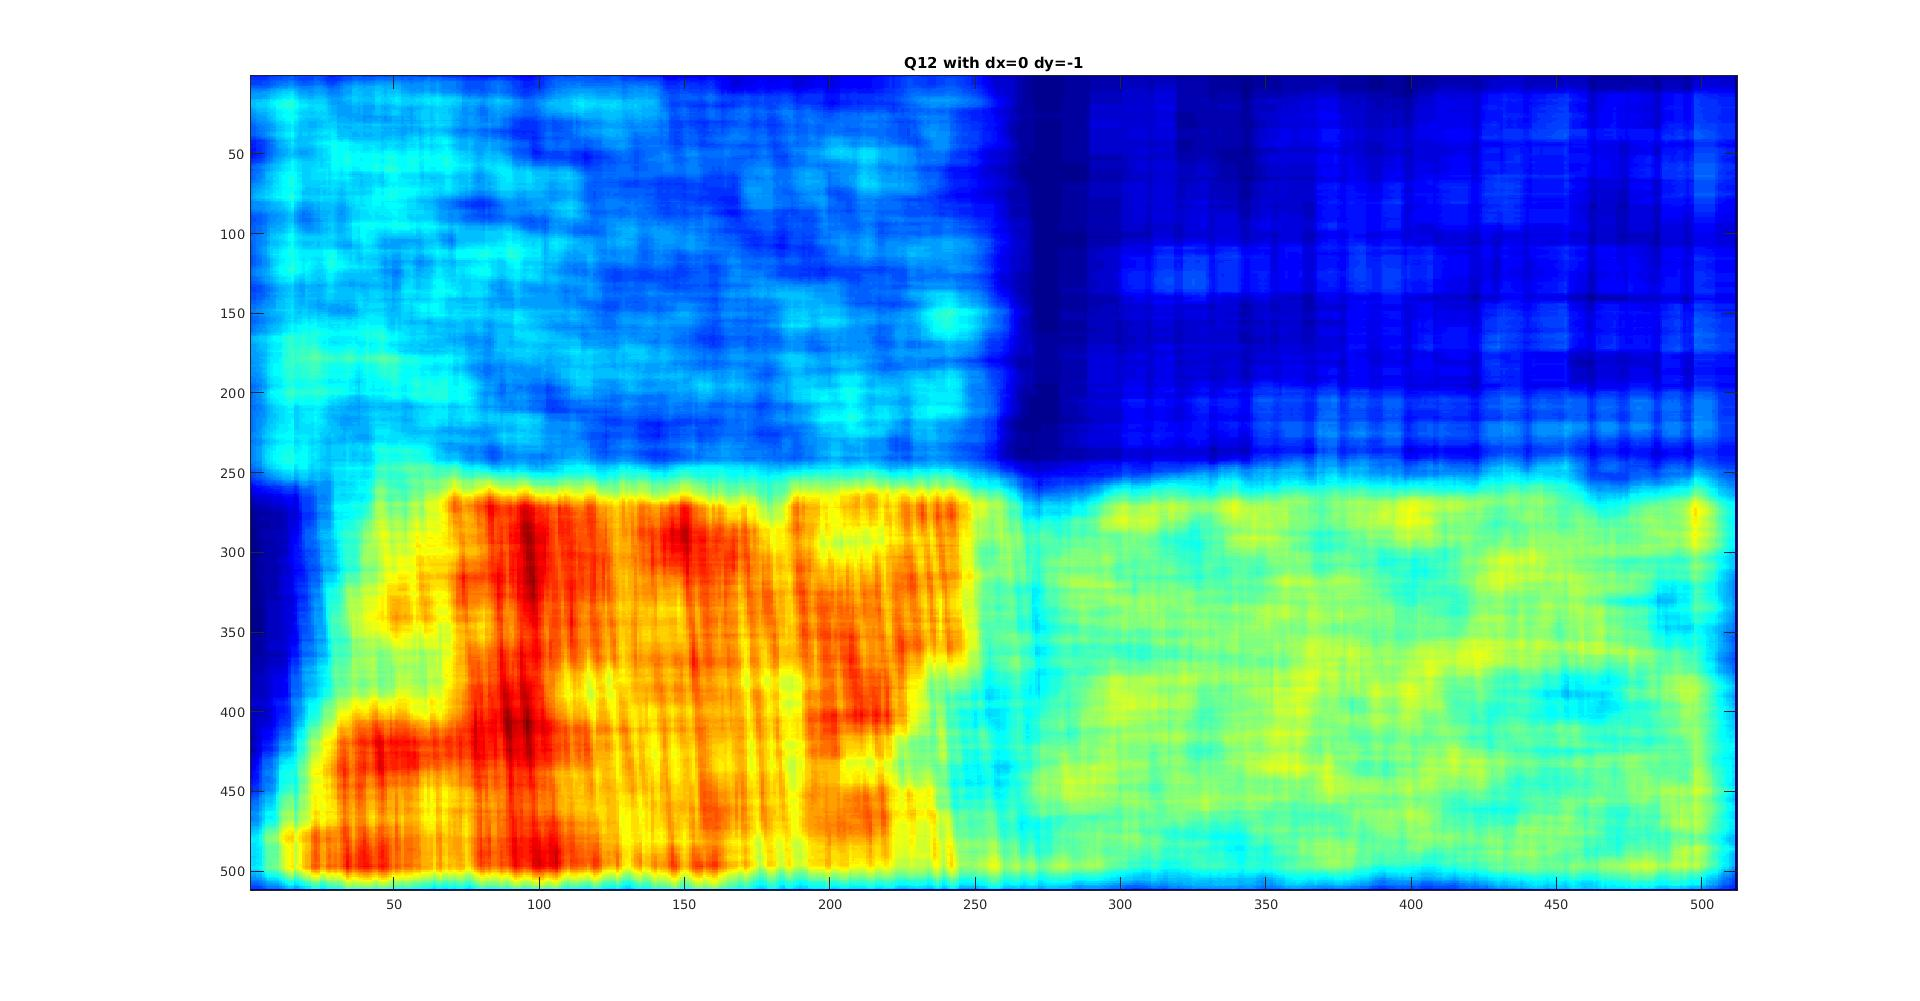
\includegraphics[width=12.5cm]{o3_q12.jpg} }}%
    	\caption{TQadrant Q12 with dx=0 and dy=-1}%
    	\label{fig:o3_q12}%
	\end{figure}
The last quadrant is chosen mainly for the recognition of the bottom left texture.\\
\vspace{10px}
We now have 3 features to differentiate the textures. We can now work on the Multivariate Gaussian Classifier to train and recognize the textures. 


\section{Multivariate Gaussian Classifier}	
		After we got the GLCM matrix for the 3 different values, our next next task is to use a Multivariate Gaussian Classifier to try to classify the 4 patterns.\\
	After the features was identified we ran it on the training mask to extract the $\mu$ and $\sigma$.\\
	$\mu$ is the mean of the classes, and $\sigma$ us the covariance of all the features for all 4 classes.\\
	With these values we can calculate the Multivariate Gaussian Classifier.
	The formula for Multivariate Gaussian Classifier (in multiple dimensions) is:
	\begin{center}
		$y = f( x , \mu , \sigma)=\frac{1}{\sqrt{|\sigma|(2\pi)^{d}}}exp\left(-\frac{1}{2}(x-\mu)\sum^{-1}(x-\mu)'\right)$
	\end{center}
	
\newpage
\section{Classification}
After running the classifier on the first training set the result was this:
\begin{figure}[h!]%
		\centering
    	\subfloat[Probability of class 1]{{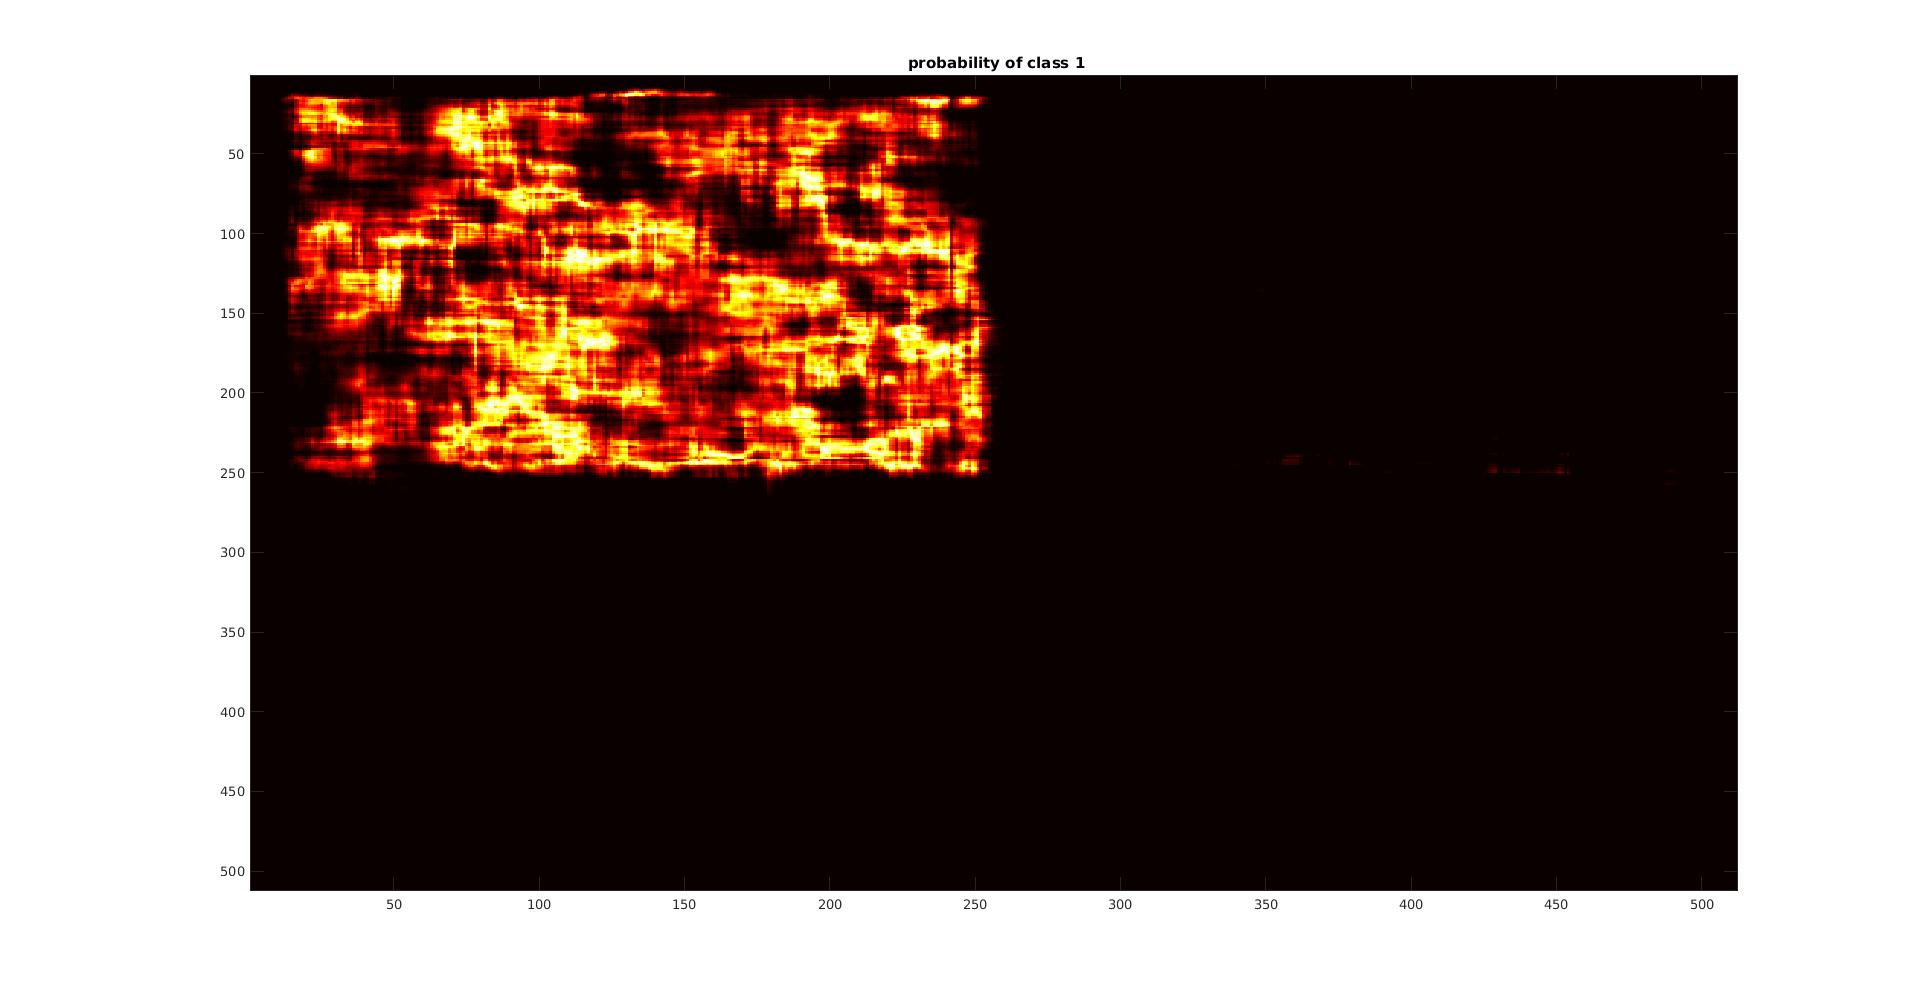
\includegraphics[width=5.5cm]{class1.jpg} }}%
    	\subfloat[Probability of class 2]{{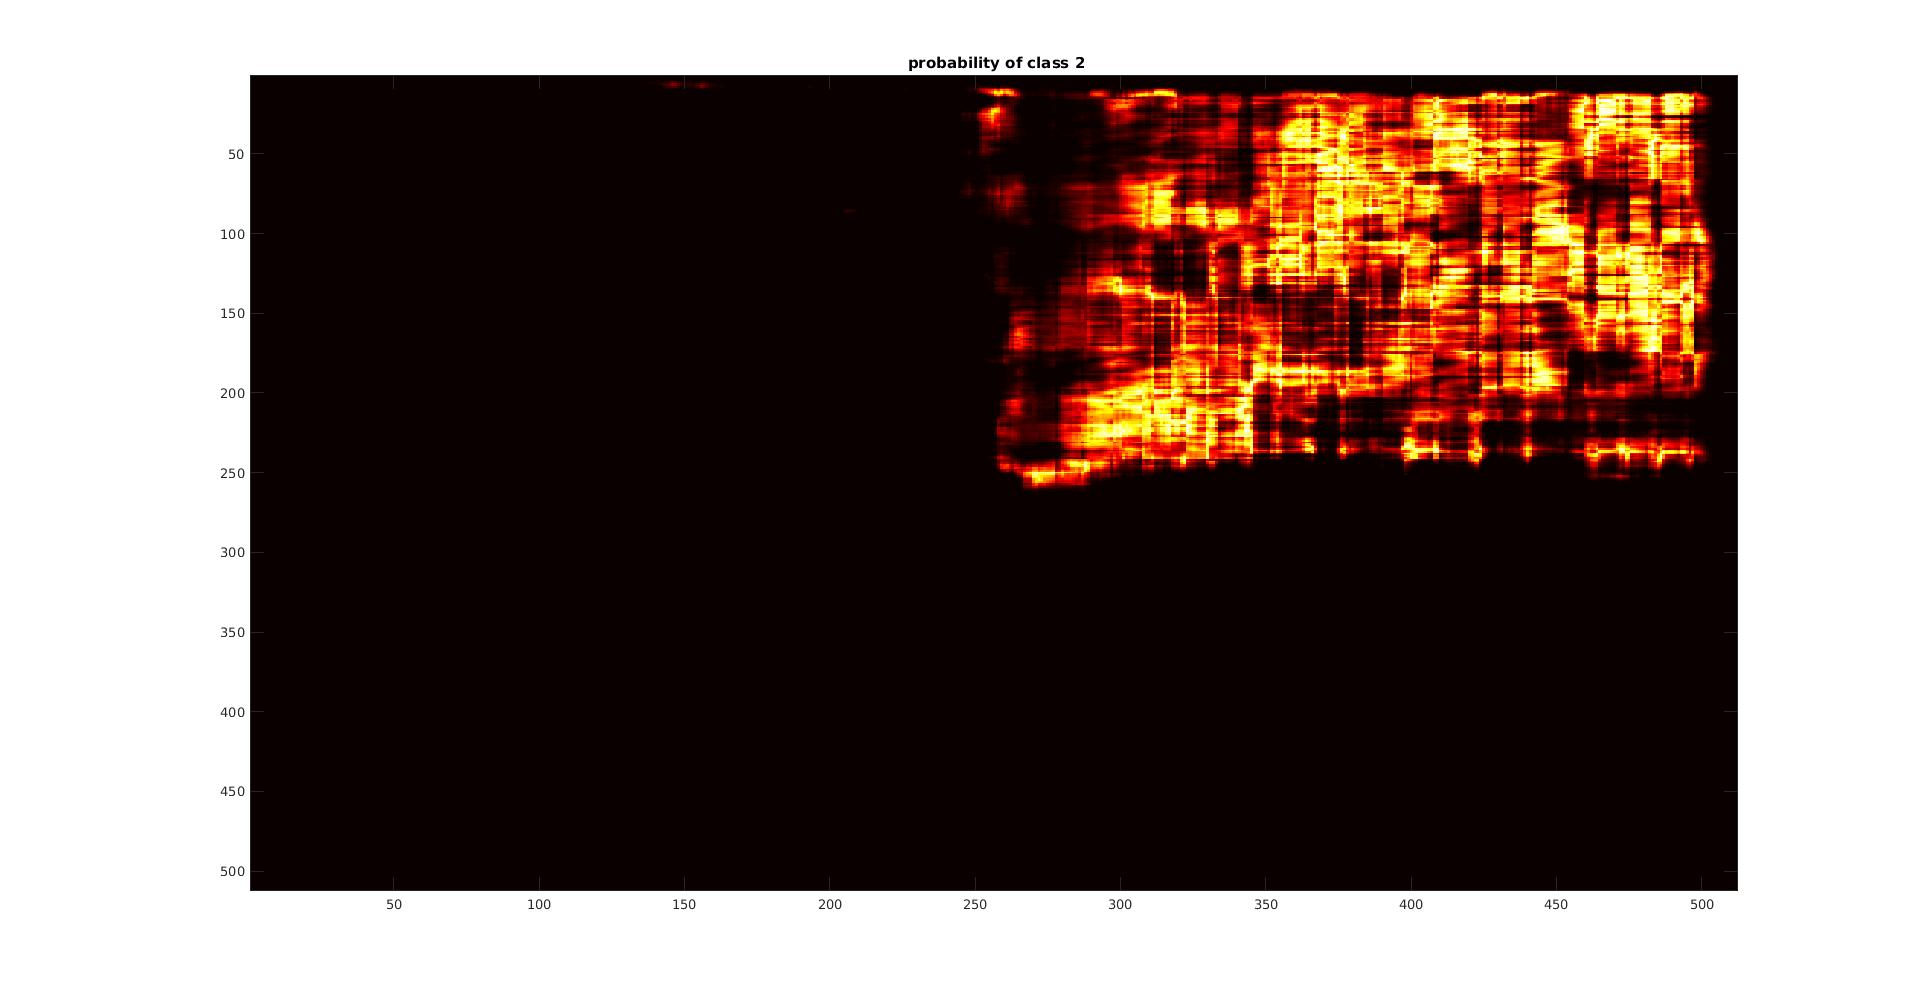
\includegraphics[width=5.5cm]{class2.jpg} }}%
    	\caption{2 first classifiers }%
	
    	\label{fig:p12}%
	\end{figure}
\begin{figure}[h!]%
		\centering
    	\subfloat[Probability of class 3]{{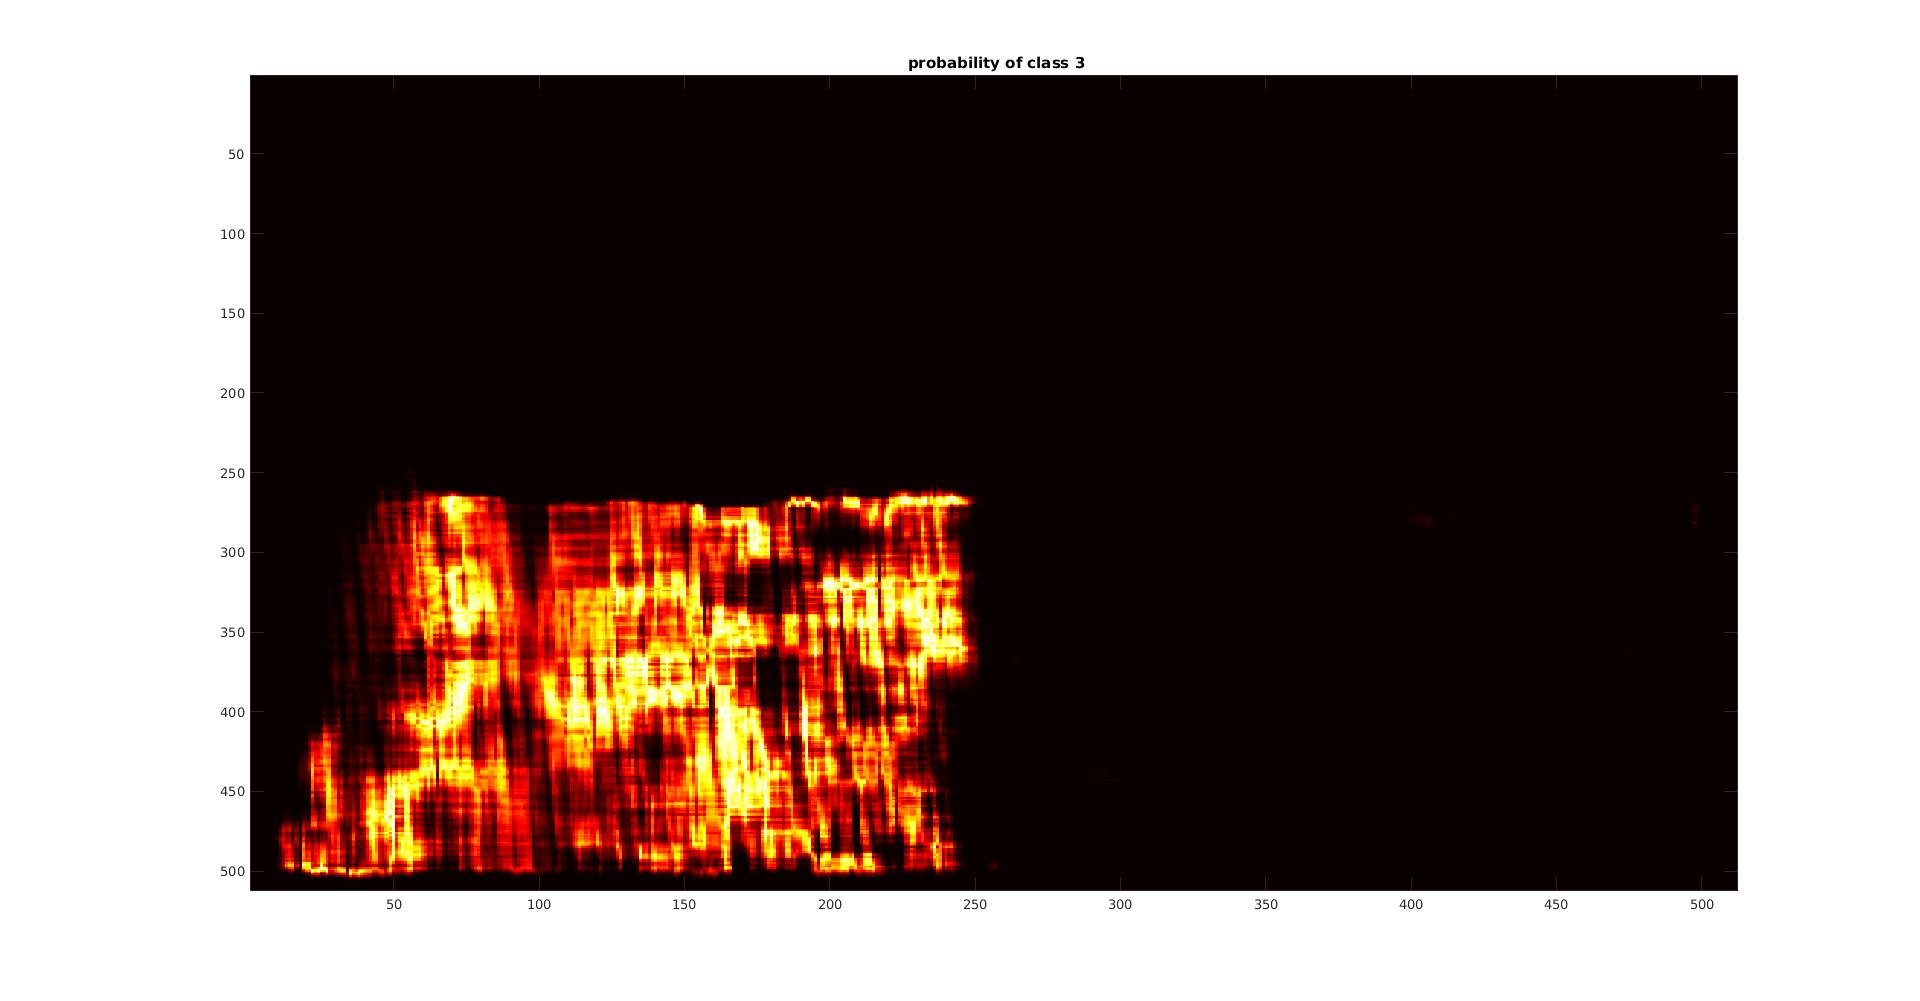
\includegraphics[width=5.5cm]{class3.jpg} }}%
    	\subfloat[Probability of class 4]{{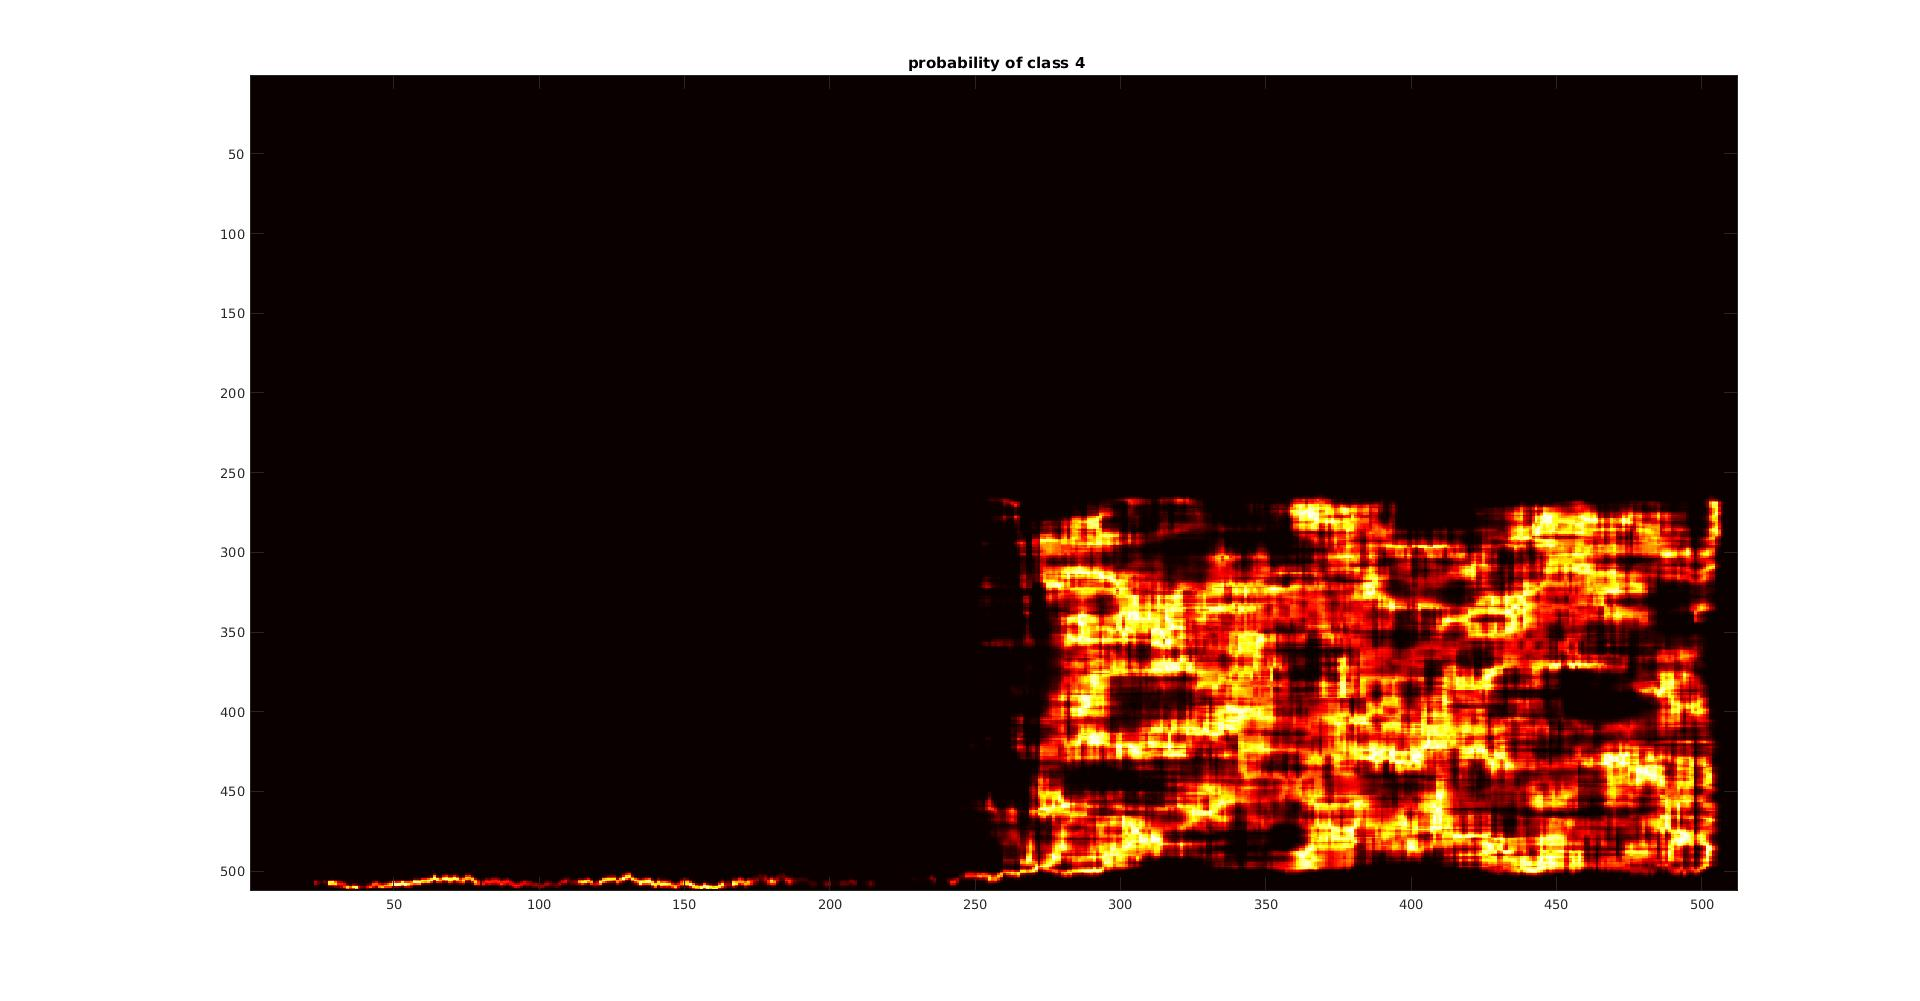
\includegraphics[width=5.5cm]{class4.jpg} }}%
    	\caption{2 last classifiers }%

    	\label{fig:p34}%
	\end{figure}


\newpage
\section{Testing}
	
\begin{comment}

	\subsection{The discarded result}
	Getting a good result varies a lot on the GLCM matrix that we chose early in the process.
	This is a result that i chose to discard, where the GLCM matrices had different values than the one i ended up with.	
	
	\begin{figure}[h]
	\centering
	\begin{BVerbatim}
confusion =
       56294        1661        4562         513
         378       58446         725          36
        8353        5428       53798       15786
           0           0        6450       49714
acc =
   83.2565

confusion =
       56610        2273        2883         522
        1205       54745         267           0
        7210        8517       56017       14861
           0           0        6368       50666
acc =
   83.1749

confusion =
       39056       18547       15736        9122
       12458       38550        3086       25138
       13511        8438       46573       31637
           0           0         140         152
acc =
   47.4285

	\end{BVerbatim}
	\caption{Result from a run with dx=0 dy=-1 and dx=1 dy=0}%
	\label{verb:wrongGLCM}
	\end{figure}
	Here we have almost 50\% on the last test, which is higher than the one that i ended up with, but it failed to find any of the pattern from the bottom right corner. 
	

\end{comment}\\


	\subsection{The final result}
	The dx/dy values with the chosen quadrants yielded the following result: 
\begin{comment}
\begin{figure}[h]
	\centering
	\begin{BVerbatim}
confusion =
           0           0         255         255         513
           0       59360        1594        1034        1070
           0        4223       63678         317         724
           0         140           8       60413         788
           0        1302           0        3516       62954
acc =
   93.9960

confusion =
           0           0         255         255         513
           0       58573        1866        5321	 	 857
           0        4824       63374         401    	1024
           0         415          24       54001    	2084
           0        1213          16        5557   	   61571
acc =
   90.6063

confusion =
           0           0         255         255         513
           0       55720       44913       15930        4903
           0        8506       19448        5213       46792
           0         357          32       38357         305
           0         442         887        5780       13536
acc =
   48.4699
	\end{BVerbatim}
	\caption{Result from a run with dx=1 dy=0 and dx=0 dy=-1 (opposite of the other result) }%
	\label{verb:rightGLCM}
	\end{figure}
	
	\end{comment}

\newpage
\subsection{Training set}
	The training set gave us
	\begin{figure}[h!]%
		\centering
    	\subfloat[Texture 4]{{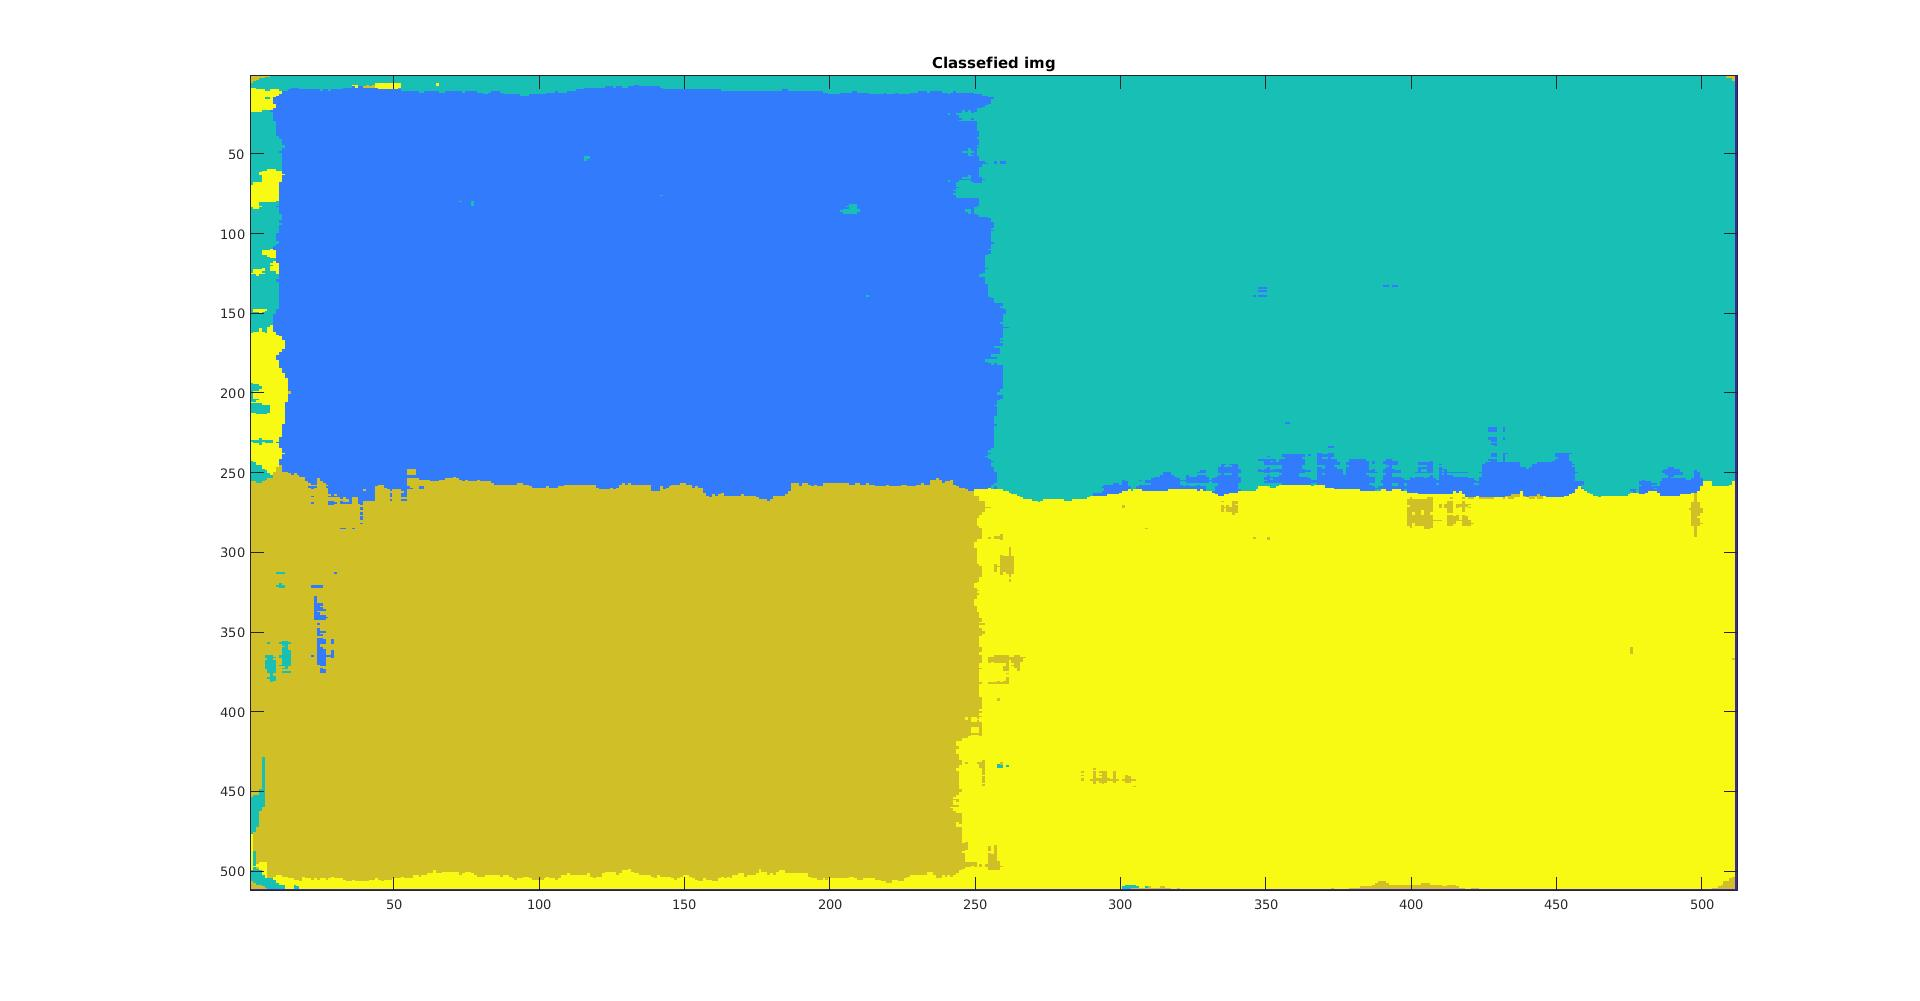
\includegraphics[width=12.5cm]{final_clas.jpg} }}%
    	\caption{Final classification after training}%
    	\label{fig:f0}%
	\end{figure}
	
\vspace{10px}
\begin{table}
\centering
Confusion Matrix\\
\begin{tabular}{c | c | c | c | c}
 0  & 0     & 255   & 255   & 513 \\\hline
 0  & 59360 & 1594  & 1034  & 1070 \\\hline
 0  & 4223  & 63678 & 317   & 724 \\\hline
 0  & 140   & 8     & 60413 & 788 \\\hline
 0  & 1302  & 0     & 3516  & 62954 \\\hline
\end{tabular}
\caption {Accuracy: 93.9960\%}
\end{table}

	As we can see, the training data is close to perfect, as expected. 
		
	\newpage
\subsection{Test set 1}
	\begin{figure}[h!]%
		\centering
    	\subfloat[Texture 4]{{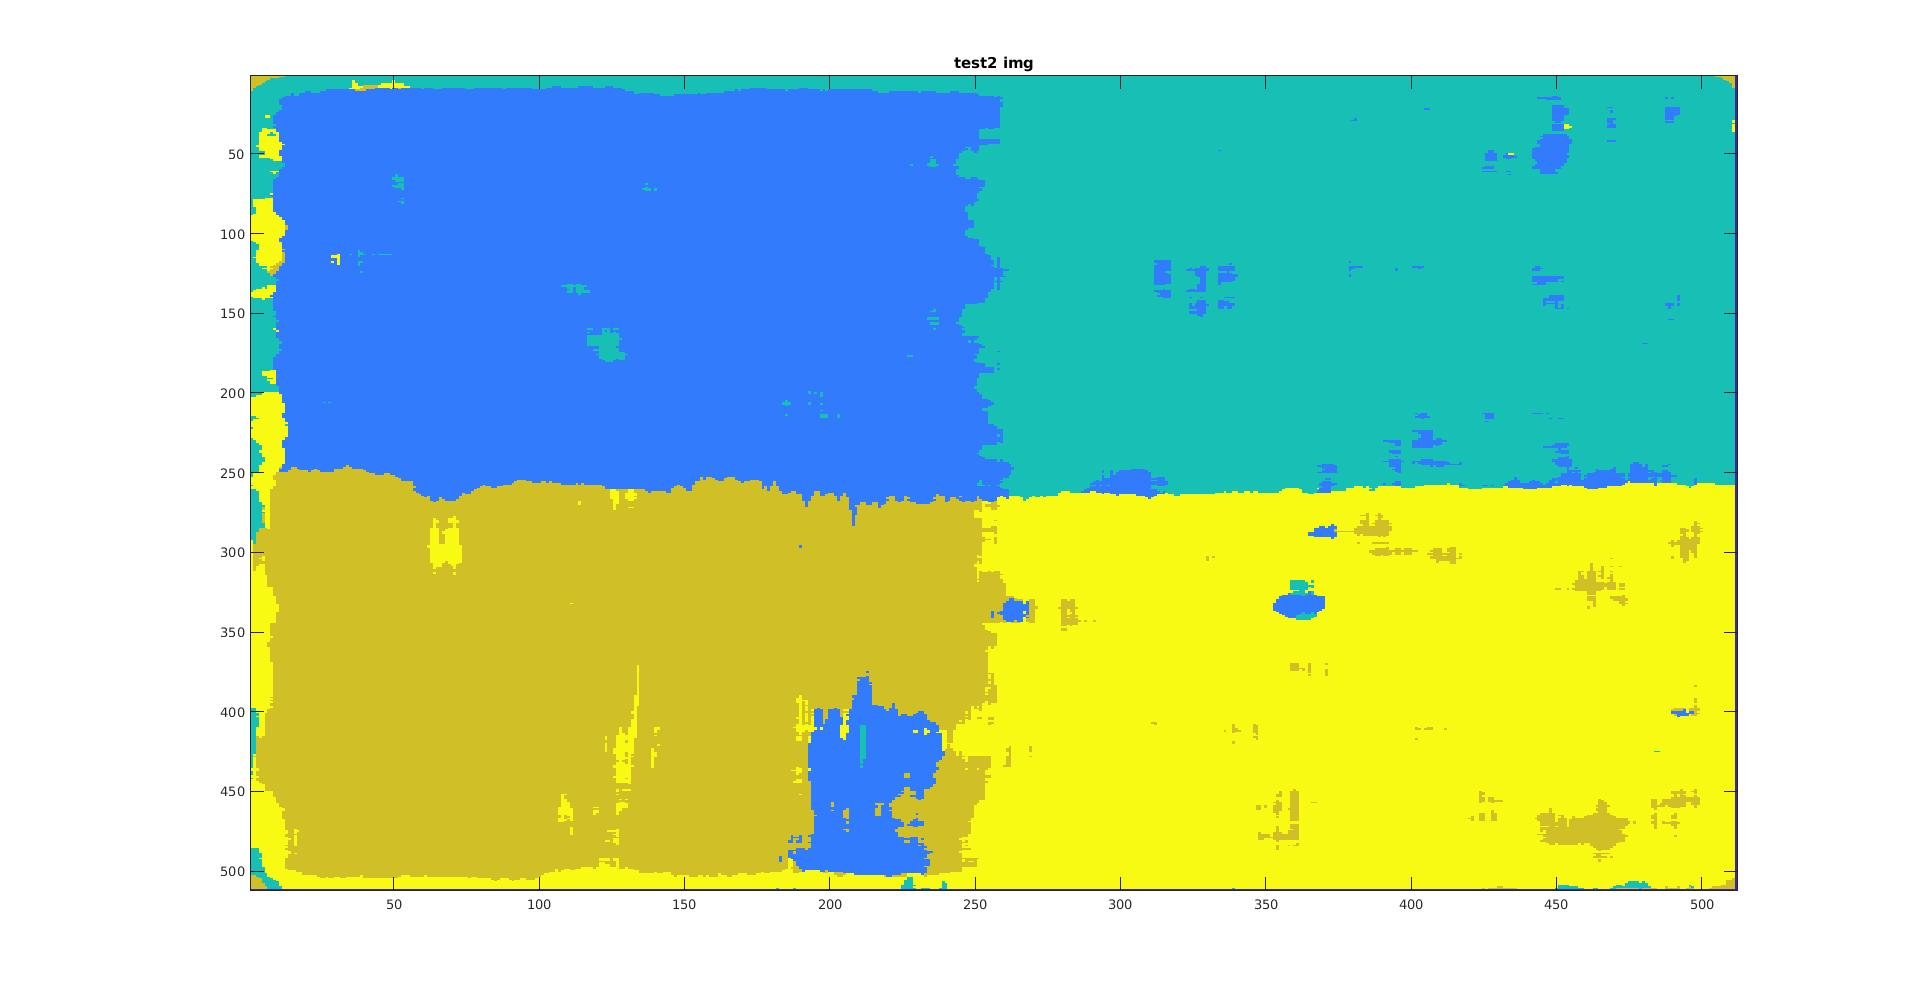
\includegraphics[width=12.5cm]{final_t1.jpg} }}%
    	\caption{Test classification on test number 1}%
    	\label{fig:f1}%
	\end{figure}
\begin{table}
\centering
Confusion Matrix\\
\begin{tabular}{c | c | c | c | c}
 0  & 0     & 255   & 255   & 513   \\\hline
 0  & 58573 & 1866  & 5321  & 857   \\\hline
 0  & 4824  & 63374 & 401   & 1024  \\\hline
 0  & 415   & 24    & 54001 & 2084  \\\hline
 0  & 1213  & 16    & 5557  & 61571 \\\hline
\end{tabular}
\caption {Accuracy: 90.6063}
\end{table}

	Here we got some trouble in class 3. Everything else is really close. Good enough result.
	\newpage 
\subsection{Test set 2}

	\begin{figure}[h!]%
		\centering
    	\subfloat[Texture 4]{{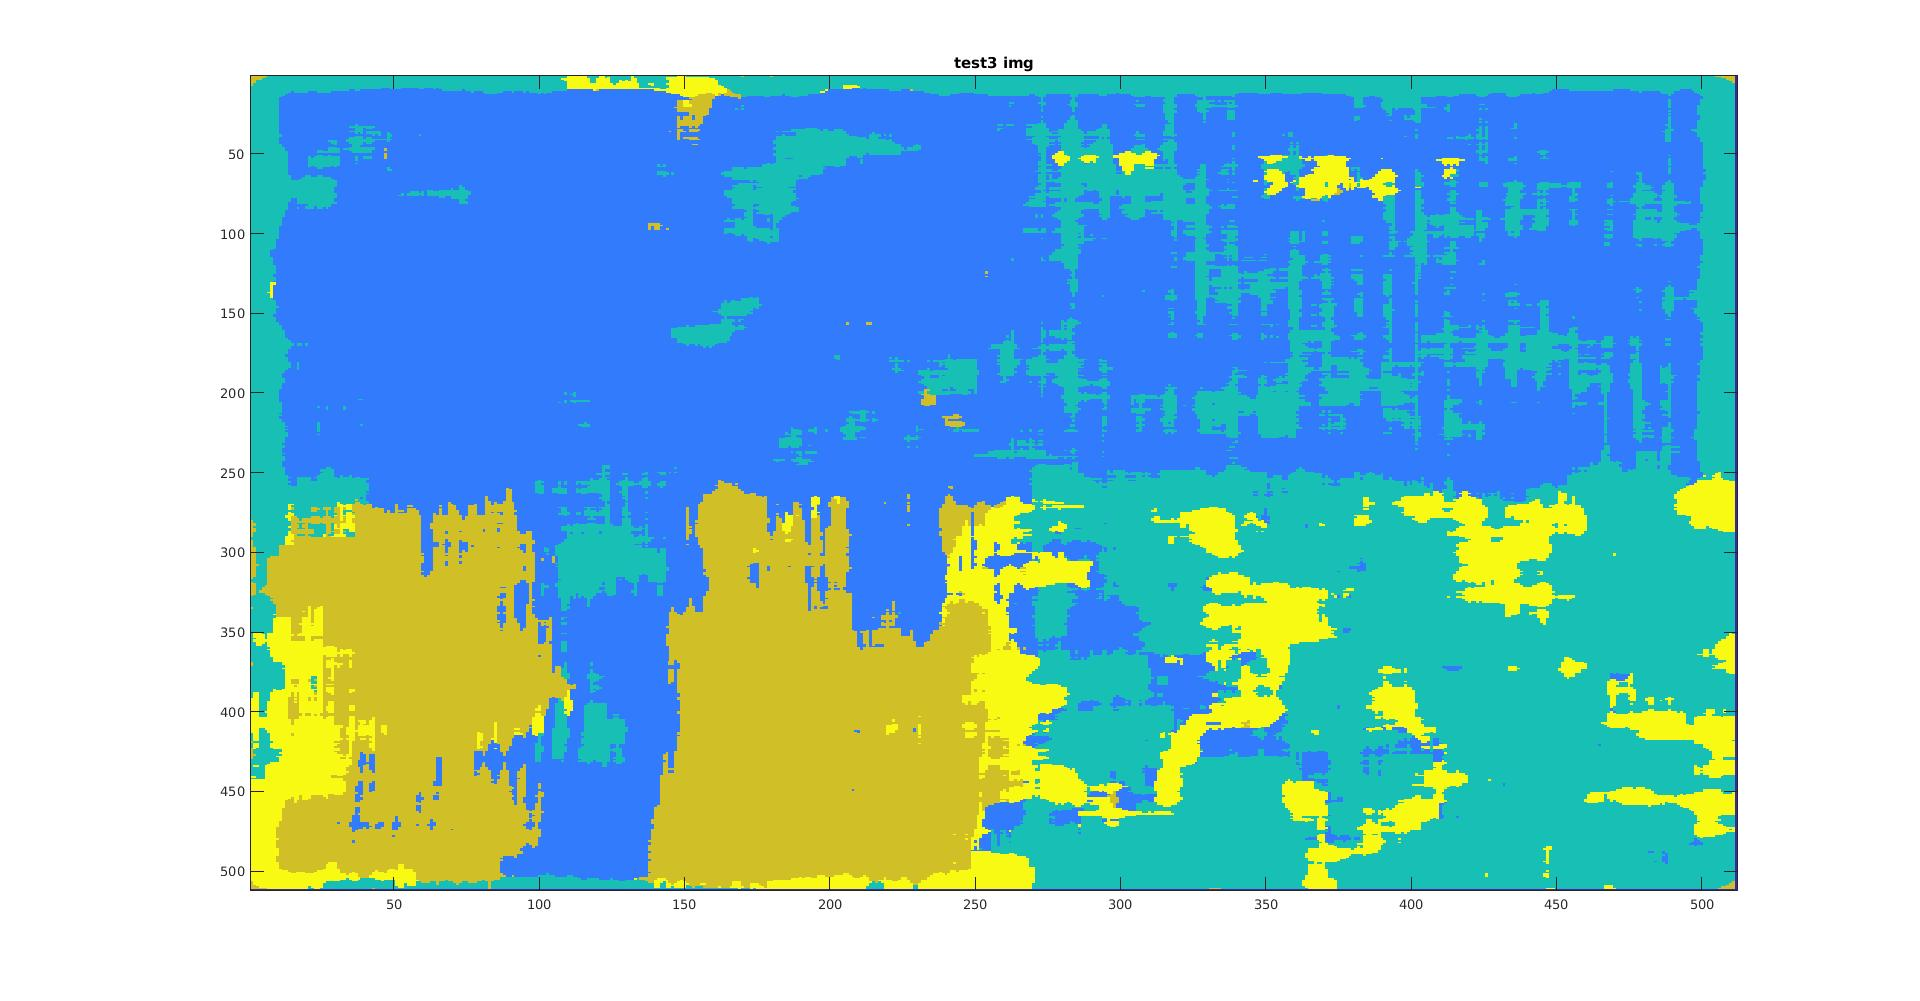
\includegraphics[width=12.5cm]{final_t2.jpg} }}%
    	\caption{Test classification on test number 2}%
    	\label{fig:f2}%
	\end{figure}
	\begin{table}
\centering
Confusion Matrix\\
\begin{tabular}{c | c | c | c | c}
  0  & 0     & 255   & 255   & 513   \\\hline
  0  & 55720 & 44913 & 15930 & 4903  \\\hline
  0  & 8506  & 19448 & 5213  & 46792 \\\hline
  0  & 357   & 32    & 38357 & 305   \\\hline
  0  & 442   & 887   & 5780  & 13536 \\\hline
\end{tabular}
\caption {Accuracy: 48.4699\%}
\end{table}
	At this point the test is to warped to get a desirable result. We end up at almost 50 percent, which isn't too bad.


\newpage
\newpage
\newpage


\section{appendix A - Gliding GLCM}
	First, the gliding GLCM
	\lstinputlisting[language=Matlab]{../files/gGLCM.m}

	\newpage
\section{appendix B - Main program}
	\lstinputlisting[language=Matlab]{../files/oblig2.m}

	\newpage
\section{appendix C - Classifier}
	Third, the classifier 
	\lstinputlisting[language=Matlab]{../files/oppg7.m}
    


\end{document}\\

